% !TEX program = xelatex
\documentclass{InforMeX}

\begin{document}
\sloppy
\portada{Máster en Ingeniería de Sistemas y Control}
{Prácticas de Computación y Robótica}
{Javier Arambarri Calvo}
{2025/2026}
{\today}
{Proyecto}

%%%%%%%%%%%%%%%%%%%%
% \datos{1}{2}{3}
%  1- color -> imprime logo en color; cc-> imprime logo en B/N
%  2- Título del documento
%  3- Nombre del Vicerrectorado
%%%%%%%%%%%%%%%%%%%%
\datos{color}{}{}
\section*{Autoría}

\textit{El autor de este documento es Javier Arambarri Calvo, alumno del Máster en Ingeniería de Sistemas y Control y matriculado por la Universidad Complutense de Madrid en el curso académico 2025-2026.}\\

\textit{Para que así conste, se firma digitalmente este documento.}

\renewcommand{\tablename}{Tabla}
\renewcommand{\listtablename}{Índice de tablas}


\datos{color}{}{}
\tableofcontents
%\newpage
\listoffigures
%\newpage
\listoftables
%\lstlistoflistings

\newpage
%%%%%%%%%%%%%%%%%%%%
% \adaptar{1}{2}
% 1- Si -> aumentar tamaño de letra
% 2- Si -> Adaptado con colores de Baja Visión
%%%%%%%%%%%%%%%%%%%%
\adaptar{no}{no}

\datos{color}{}{}
\section{Enunciado}
%\addcontentsline{toc}{section}{Ejercicio 1}
En este tema se plantea un único ejercicio de investigación cuyo objetivo es clasificar
diversos tipos de robots de acuerdo a los conceptos introducidos en el desarrollo teórico
del tema. \\

El trabajo consiste en la búsqueda por medio de internet u otras fuentes de información
de al menos un ejemplo real de robot de cada uno de los tipos y arquitecturas mostrados
en la teoría. \\

De este modo deberá haber al menos un robot que tenga una arquitectura centralizada,
un robot con arquitectura distribuida y otro con arquitectura híbrida. Además tendrá que
haber al menos un robot con ruedas, un robot con cadenas, un robot con patas y un robot
marino o aéreo. También deberá ponerse algún ejemplo de robot colaborativo o de red
de sensores. \\

Para facilitar la corrección y la verificación por parte del alumno de que se están
cubriendo todos los tipos y arquitecturas debe rellenarse una tabla de la forma siguiente, 
Figura \ref{fig:tablaEnunciado}.

\begin{figure}[htb]
    \centering
    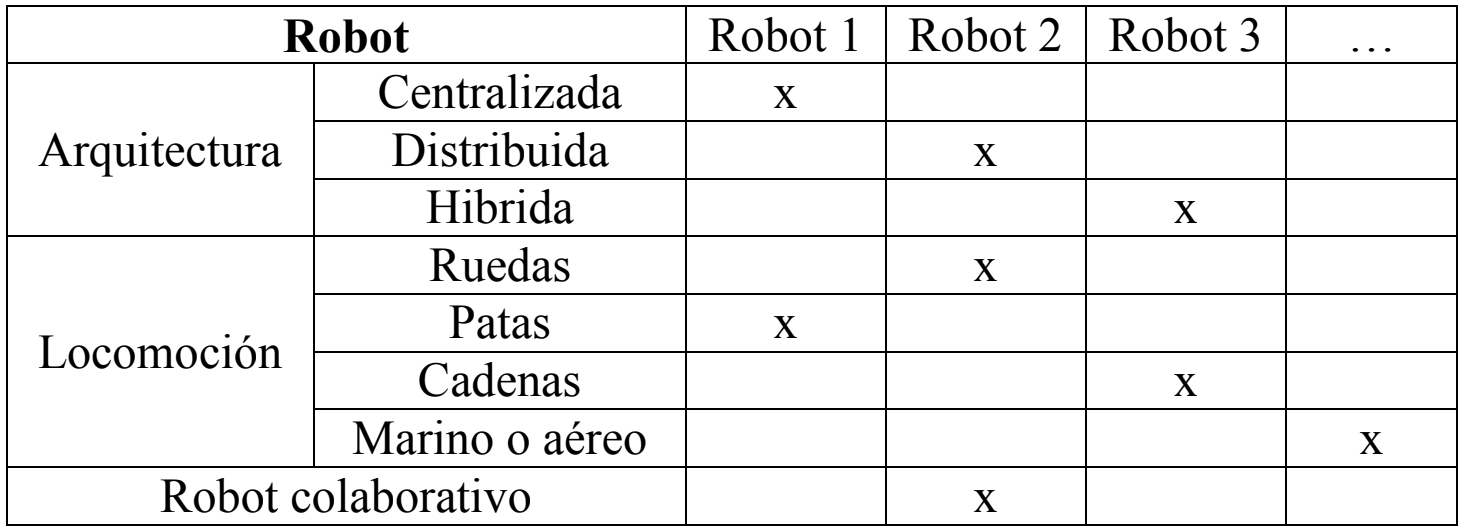
\includegraphics[scale=0.29]{Images/tablaEnunciado.png}
    \caption{Tabla a rellenar} \label{fig:tablaEnunciado}
\end{figure}

Para cada uno de los robots habrá que completar una pequeña ficha que contenga la
siguiente información.
\begin{itemize}
    \item Nombre.
    \item Breve descripción del robot.
    \item Uso(s) principal(es) del robot.
    \item Breve descripción de la arquitectura del robot.
    \item Breve descripción del método de locomoción.
    \item Empresa, entidad u organismo que lo ha construido.
    \item Fotografía del robot.
    \item Referencias (URLs o Referencias a libros o revistas donde pueda verificarse tal
información). \\
\end{itemize}

La ficha del robot no pretende ser una descripción exhaustiva, puesto que lo que se
pretende es comprobar que se han comprendido correctamente los tipos de robots y
arquitecturas existentes. Por este motivo el espacio destinado a la ficha de cada robot no
debe exceder una cara.
\datos{color}{}{}
\section*{Tarea 1: experimento de control de posición de un robot móvil.}
\addcontentsline{toc}{section}{Tarea 1: experimento de control de posición de un robot móvil.}

El experimento consiste en controlar la posición de un robot móvil con el
Simulador CoppeliaSim. Los pasos a llevar a cabo son los siguientes:

\subsection*{1. Descargar el simulador y agregar el modelo del robot al mismo como se
explica en el documento Interfaz de la Práctica.}
\addcontentsline{toc}{subsection}{1. Descargar el simulador y agregar el modelo del robot al mismo como se
explica en el documento Interfaz de la Práctica.}

Se ha creado una imagen de \textit{Docker} con el simulador instalado, el modelo del robot
\textit{Khepera IV}, y el \textit{framework ROS2}. En el apartado \ref{} se detalla la descarga 
e instalación utilizando \textit{Docker}. En la Figura \ref{fig:t1.2} se observa que el robot se 
ha cargado correctamente.

\subsection*{2. Al arrastrar el robot desde el panel lateral y soltarlo en el espacio de
trabajo, el robot quedará agregado a la simulación.}
\addcontentsline{toc}{subsection}{2. Al arrastrar el robot desde el panel lateral y soltarlo en el espacio de
trabajo, el robot quedará agregado a la simulación.}

En la Figura \ref{fig:t1.2} se observa que el robot se 
ha agregado correctamente a la simulación.

\begin{figure}[H]
    \begin{center}
    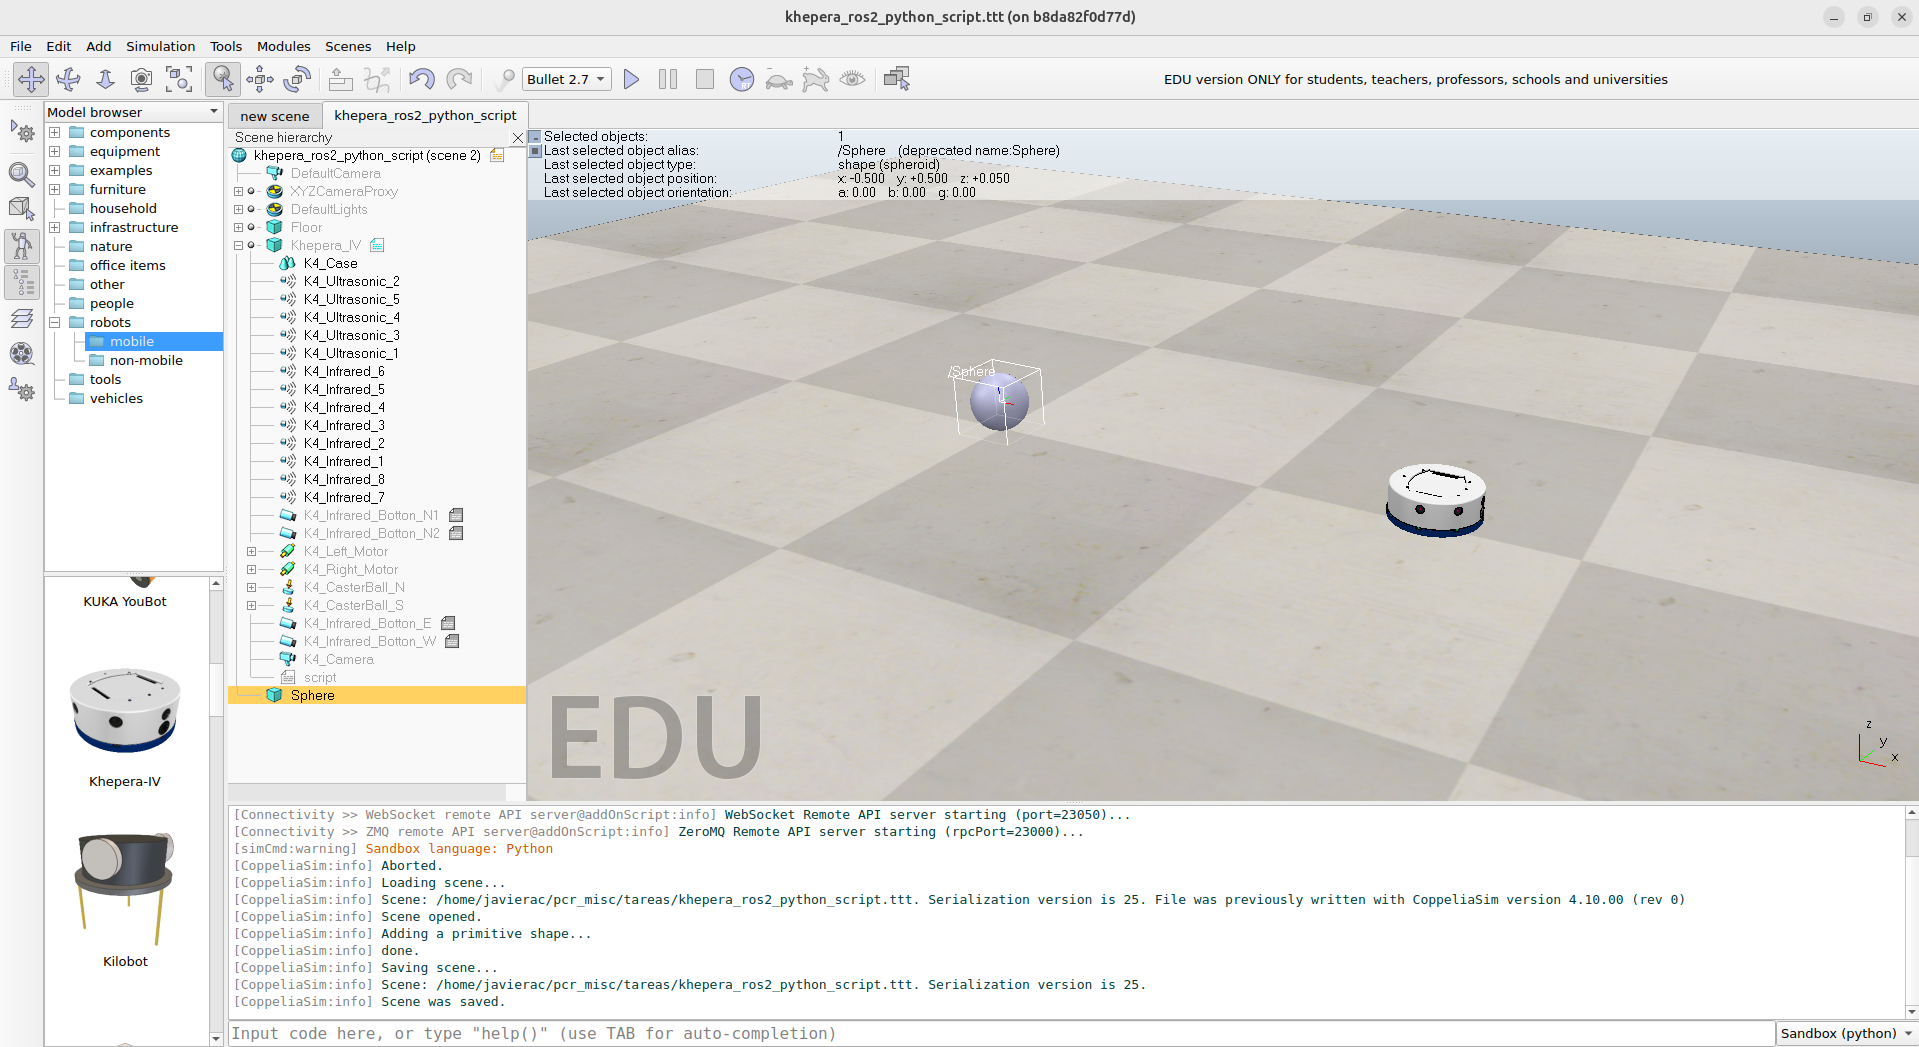
\includegraphics[scale=0.2, angle=0]{Images/tarea1/robot.png}
    \caption{\label{fig:t1.2} Robot \textit{Khepera IV} y objeto que representa el
    punto de destino agregados a \textit{Coppelia Sim}.}
    \end{center}
\end{figure}

\subsection*{3. Iniciar la simulación y observar el comportamiento del robot. ¿A qué se
debe este comportamiento?}
\addcontentsline{toc}{subsection}{3. Iniciar la simulación y observar el comportamiento del robot. ¿A qué se
debe este comportamiento?}

\subsection*{4. Abrir el script de programación del robot y observar los valores de las
velocidades izquierda y derecha.}
\addcontentsline{toc}{subsection}{4. Abrir el script de programación del robot y observar los valores de las
velocidades izquierda y derecha.}

El robot se mueve dibujando una trayectoria en arco de circunferencia, Figura \ref{fig:t1.3_2}. Haciendo doble click en el script por defecto del robot,
Figura \ref{fig:t1.3}, se abre el script que se presenta en el Código \ref{cod:t1.3}. Este comportamiento
se debe a las velocidades angulares ($w_L,\; w_R$) asignadas a cada motor: 3 rad/s al izquierdo y 5 rad/s al derecho,
respectivamente. Por tanto, el motor izquierdo gira más lento que el derecho y el robot realiza una trayectoria
en arco de circunferencia de radio $R = 0.176 \text{ metros}$, que se obtiene mediante la Ecuación (1) conociendo
la distancia entre los centros de las ruedas (\textit{axle track}), $L = 0.088 \text{ metros}$.

\begin{equation}
R = \frac{L}{2} \cdot \frac{\omega_R + \omega_L}{\omega_R - \omega_L}
\end{equation}

\begin{figure}[H]
    \centering

    \begin{minipage}{0.48\textwidth}
        \centering
        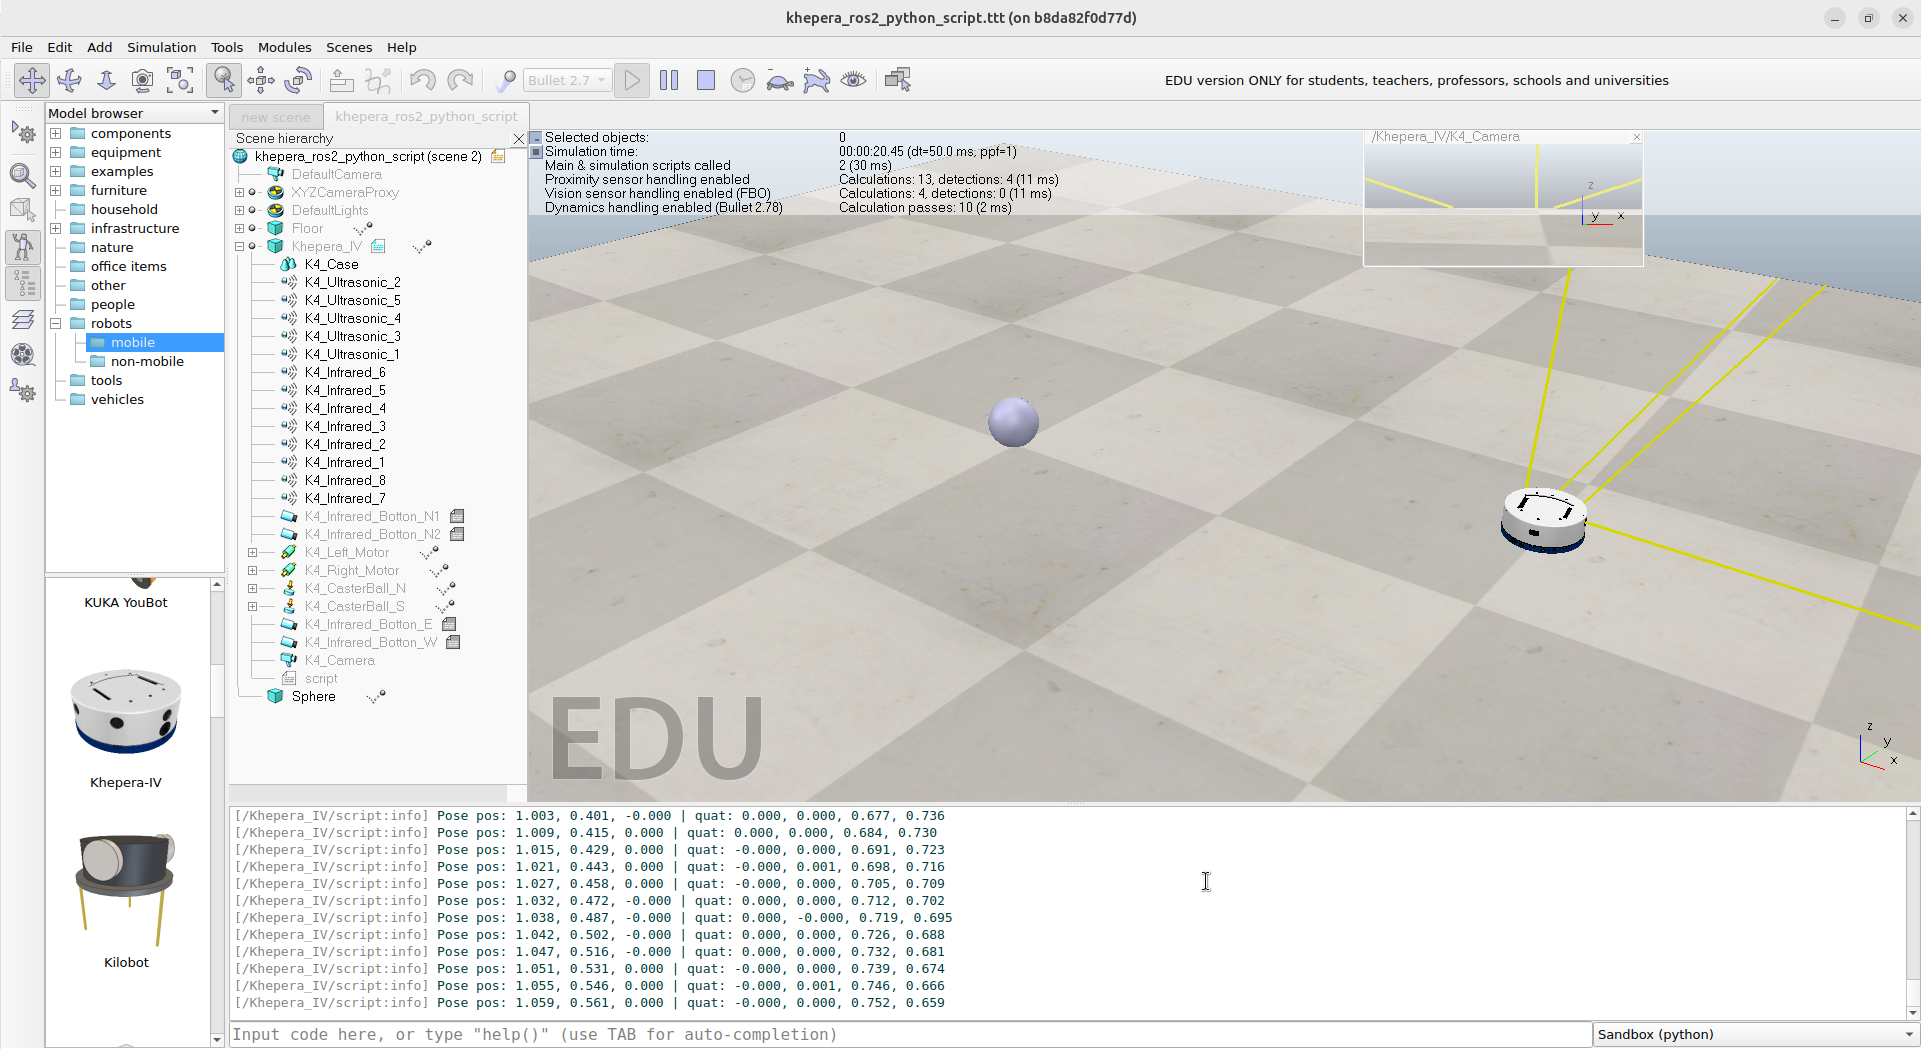
\includegraphics[scale=0.16]{Images/tarea1/trayectoria_por_defecto.png}
        \caption{\label{fig:t1.3_2} Trayectoria por defecto.}
    \end{minipage}
    \hfill
    \begin{minipage}{0.35\textwidth}
        \centering
        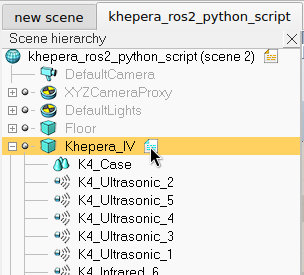
\includegraphics[scale=0.5]{Images/tarea1/script.png}
        \caption{\label{fig:t1.3} Script por defecto del robot.}
    \end{minipage}

\end{figure}

\begin{comment}
    \begin{figure}[H]
    \begin{center}
    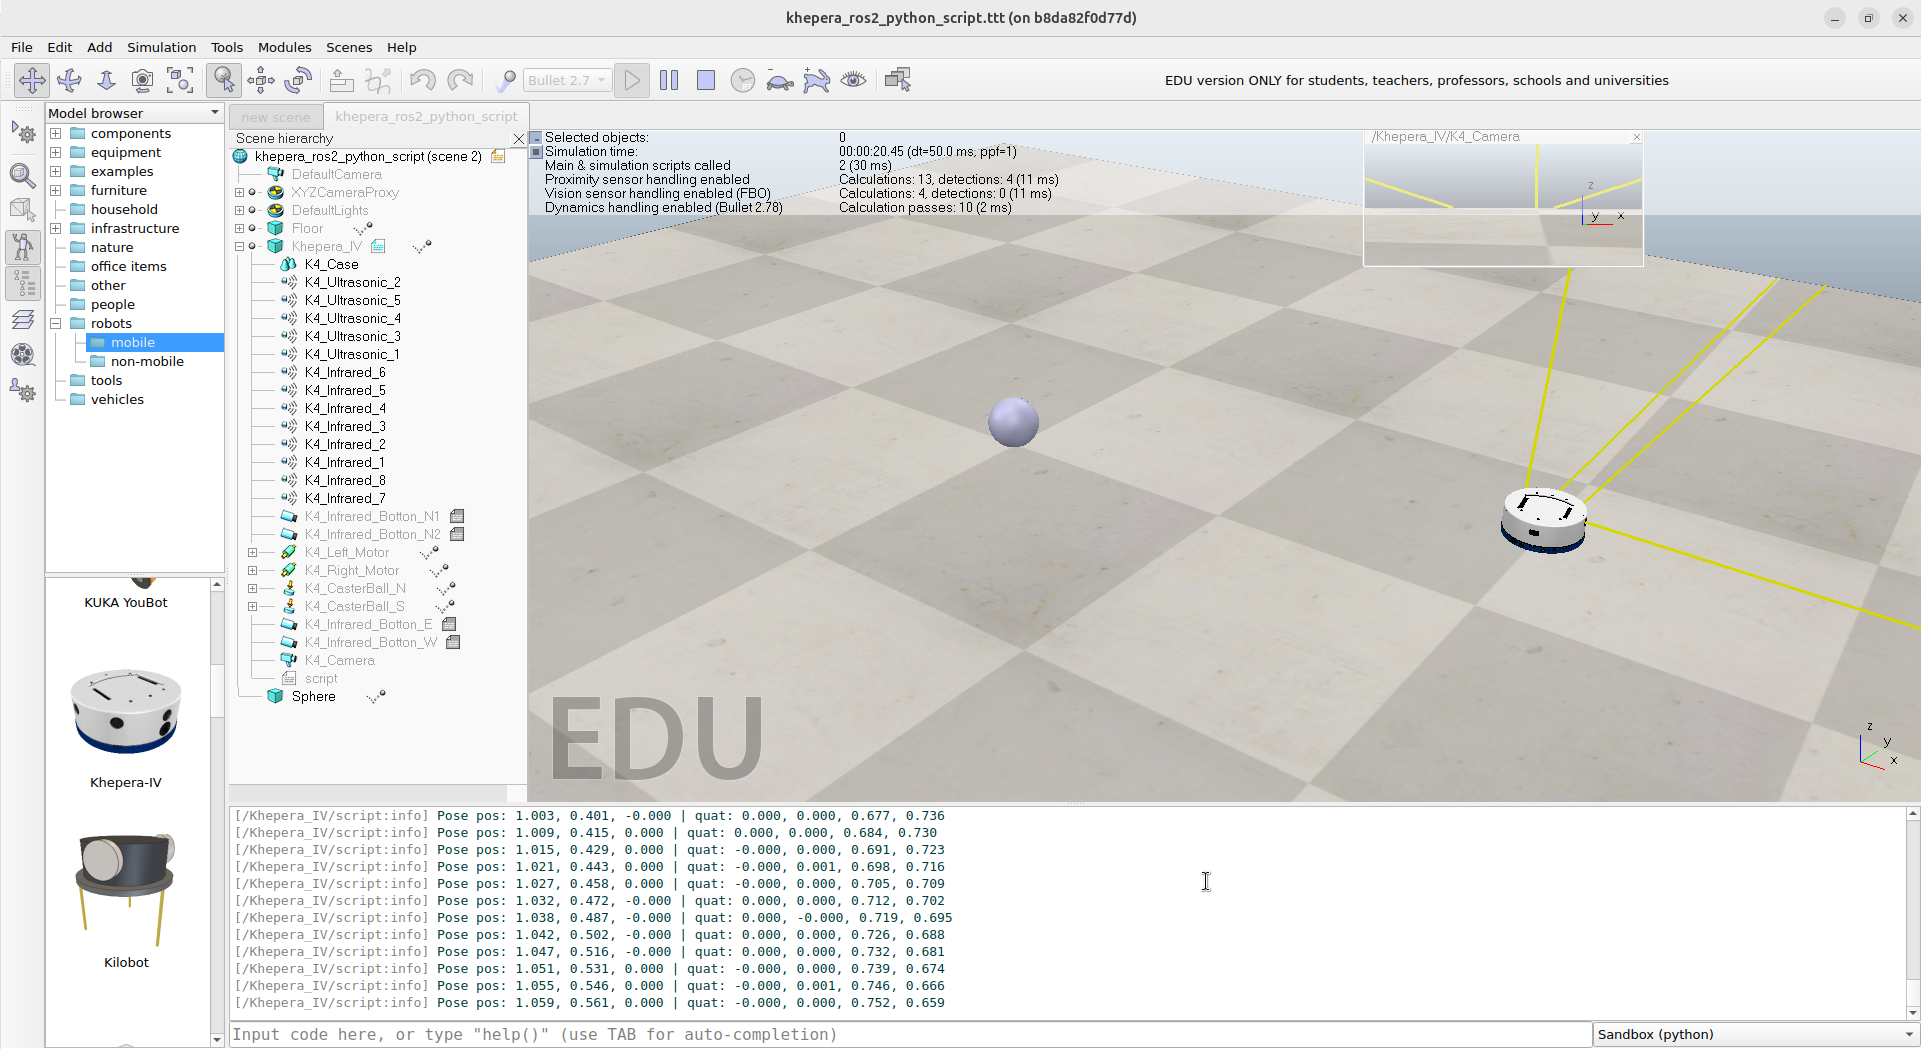
\includegraphics[scale=0.5, angle=0]{Images/tarea1/trayectoria_por_defecto.png}
    \caption{\label{fig:t1.3_2} Trayectoria por defecto.}
    \end{center}
\end{figure}

\begin{figure}[H]
    \begin{center}
    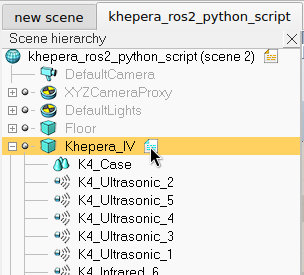
\includegraphics[scale=0.5, angle=0]{Images/tarea1/script.png}
    \caption{\label{fig:t1.3} Script por defecto del robot.}
    \end{center}
\end{figure}
\end{comment}

\lstinputlisting[style=luastyle, caption={Script por defecto del robot.}, label={cod:t1.3}]{Code/tarea1/script_por_defecto.lua}


\subsection*{5. Agregar a la simulación un objeto que represente el punto de destino del
robot.}
\addcontentsline{toc}{subsection}{5. Agregar a la simulación un objeto que represente el punto de destino del
robot.}

Se ha añadido una esfera con las propiedades descritas en la Figura \ref{fig:t1.5} y en la posición
$(x,\; y,\; z) = (-0.5,\; 0.5,\; 0.05)$, como se observa en la Figura \ref{fig:t1.2}.

\begin{figure}[H]
    \begin{center}
    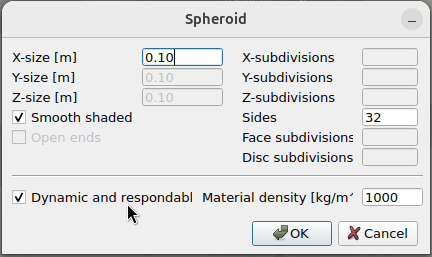
\includegraphics[scale=0.5, angle=0]{Images/tarea1/esfera.png}
    \caption{\label{fig:t1.5} Propiedades de la esfera añadida como punto de destino.}
    \end{center}
\end{figure}


\subsection*{6. Con las coordenadas del punto de destino y las del robot, calcular las
velocidades angular y lineal para controlar su posición.}
\addcontentsline{toc}{subsection}{6. Con las coordenadas del punto de destino y las del robot, calcular las
velocidades angular y lineal para controlar su posición.}

\subsection*{7. Obtener las velocidades que se envían al robot (izquierda y derecha) como
resultado del modelo diferencial. Sugerencia: se puede comenzar solamente
controlando la velocidad angular del robot a través el ángulo orientación
hacia el punto y manteniendo la velocidad lineal constante, por medio de un
control proporcional (P) sencillo. (\textit{v}=cte, \textit{w}=$\boldsymbol{K_{p}}$*(error ángulo)).}
\addcontentsline{toc}{subsection}{7. Obtener las velocidades que se envían al robot (izquierda y derecha) como
resultado del modelo diferencial.}

\subsection*{8. Implementar una ley de control diferente a la proporcionada y comparar
ambas usando los Índices de Comportamiento (IAE, ISE, ITAE, ITSE).}
\addcontentsline{toc}{subsection}{8. Implementar una ley de control diferente a la proporcionada y comparar
ambas usando los Índices de Comportamiento (IAE, ISE, ITAE, ITSE).}


\clearpage
\section{Controladores ICC para un robot diferencial}

En esta práctica se implementan y comparan dos variantes del controlador 
\textit{Instantaneous Center of Curvature} (ICC) para un robot móvil diferencial.
Ambos controladores generan velocidades lineales y angulares $(v, \omega)$
para conducir al robot desde su pose actual $(x_r, y_r, \theta_r)$ hasta un objetivo
$(x_t, y_t)$.

\subsection{Geometría del problema}

Sea la posición del robot $(x_r, y_r)$ y la del objetivo $(x_t, y_t)$.
Definimos:



\[
d = \sqrt{(x_t - x_r)^2 + (y_t - y_r)^2}
\]





\[
\theta_d = \operatorname{atan2}(y_t - y_r,\; x_t - x_r)
\]





\[
e_\theta = \theta_d - \theta_r
\]



donde $d$ es la distancia al objetivo y $e_\theta$ el error angular normalizado.

\subsection{Controlador ICC reactivo}

El controlador reactivo utiliza una ley proporcional para la velocidad lineal:



\[
v = K_v \cdot d
\]



saturada por la velocidad máxima del robot:



\[
v = \min(v,\; v_{\max})
\]



La velocidad angular se calcula como:



\[
\omega = \omega_{\max} \cdot \sin(e_\theta)
\]



Este controlador es robusto y sencillo, pero la trayectoria no es necesariamente
un arco perfecto.

\subsection{Controlador ICC geométrico}

El controlador geométrico impone que el robot siga un arco de circunferencia
que conecta su pose actual con el objetivo. La curvatura del arco viene dada por:



\[
R = \frac{d}{2 \sin(e_\theta)}
\]



La velocidad angular se obtiene directamente de la relación cinemática:



\[
\omega = \frac{v}{R}
\]



donde $v = K_v \cdot d$ como en el controlador reactivo. En este caso,
$K_v$ afecta únicamente a la rapidez del movimiento, pero no a la forma
de la trayectoria, que viene determinada por la geometría.

\section{Arquitectura del código en C++}

El proyecto se estructura en varios módulos para mejorar la claridad y la
reutilización del código:

\begin{itemize}
    \item \textbf{icc\_controller.hpp / icc\_controller.cpp}: 
    Implementa el nodo principal de ROS2, gestiona suscripciones, temporizadores,
    publicación de comandos y ejecución del bucle de control.
    
    \item \textbf{service\_utils.hpp / service\_utils.cpp}: 
    Encapsula la llamada al servicio que proporciona la posición objetivo.
    
    \item \textbf{pose\_utils.hpp}: 
    Funciones auxiliares para extraer la pose del robot y normalizar ángulos.
    
    \item \textbf{metrics\_utils.hpp / metrics\_utils.cpp}: 
    Clase encargada de registrar datos por iteración y calcular métricas globales.
\end{itemize}

El archivo \texttt{.hpp} contiene las declaraciones de clases y funciones,
mientras que los archivos \texttt{.cpp} contienen las implementaciones.
Esta separación permite compilar más rápido y mantener un código más limpio.

\section{Métricas de evaluación}

Para comparar ambos controladores se emplean métricas estándar en control:

\subsection{Integral del Error Absoluto (IAE)}



\[
\mathrm{IAE} = \int_0^T |e(t)| \, dt
\]



Penaliza el error acumulado sin considerar su magnitud cuadrática.

\subsection{Integral del Error Cuadrático (ISE)}



\[
\mathrm{ISE} = \int_0^T e(t)^2 \, dt
\]



Penaliza más fuertemente errores grandes.

\subsection{Integral del Error Absoluto Ponderado por el Tiempo (ITAE)}



\[
\mathrm{ITAE} = \int_0^T t \, |e(t)| \, dt
\]



Penaliza errores que persisten en el tiempo.

\subsection{Integral del Error Cuadrático Ponderado por el Tiempo (ITSE)}



\[
\mathrm{ITSE} = \int_0^T t \, e(t)^2 \, dt
\]



Penaliza errores grandes y tardíos, siendo útil para evaluar estabilidad.

\subsection{Implementación discreta}

Dado que el controlador opera con un periodo de muestreo $\Delta t$, las métricas
se aproximan mediante sumas:



\[
\mathrm{IAE} \approx \sum_{k=0}^{N} |e_k| \, \Delta t
\]





\[
\mathrm{ISE} \approx \sum_{k=0}^{N} e_k^2 \, \Delta t
\]





\[
\mathrm{ITAE} \approx \sum_{k=0}^{N} t_k \, |e_k| \, \Delta t
\]





\[
\mathrm{ITSE} \approx \sum_{k=0}^{N} t_k \, e_k^2 \, \Delta t
\]



Estas métricas permiten comparar objetivamente el rendimiento de ambos controladores
bajo diferentes valores de $K_v$.

\section{Registro de datos}

En cada iteración del controlador se almacena:

\begin{itemize}
    \item Tiempo $t$
    \item Pose del robot $(x_r, y_r, \theta_r)$
    \item Pose del objetivo $(x_t, y_t)$
    \item Error de distancia $d$
    \item Error angular $e_\theta$
    \item Velocidades $v$ y $\omega$
\end{itemize}

Al finalizar, se añaden las métricas globales y los parámetros utilizados
($K_v$, $v_{\max}$, $\omega_{\max}$, tipo de controlador).
Esto permite realizar comparativas rigurosas mediante tablas y gráficas.


\begin{comment}
    ICC reactivo: Control cinemático proporcional (P-control) hacia un objetivo
    Control cinemático proporcional (reactivo)
    1. Roland Siegwart, Illah Nourbakhsh, Davide Scaramuzza  
Introduction to Autonomous Mobile Robots, MIT Press, 2011.
Capítulo 6: Control of Mobile Robots.
→ Presenta controladores proporcionales para robots unicycle.

2. Bruno Siciliano, Lorenzo Sciavicco, et al.  
Robotics: Modelling, Planning and Control, Springer, 2009.
→ Sección de control cinemático de robots móviles.

3. Howie Choset et al.  
Principles of Robot Motion, MIT Press, 2005.
→ Control reactivo basado en errores de pose.

ICC geométrico: Control geométrico basado en curvatura / arco circular (Pure Pursuit puntual)
Control geométrico basado en curvatura
1. Peter Corke  
Robotics, Vision and Control, Springer, 2017.
→ Capítulo sobre Pure Pursuit y control geométrico.

2. Morin & Samson  
Motion Control of Wheeled Mobile Robots, Springer Handbook of Robotics, 2016.
→ Sección sobre control geométrico y curvatura.

3. Kanayama et al. (1990)  
“A Stable Tracking Control Method for an Autonomous Mobile Robot”, IEEE ICRA.
→ Control geométrico basado en errores de pose.

4. Coulter (1992)  
“Implementation of the Pure Pursuit Path Tracking Algorithm”, CMU.
→ Control geométrico por arco circular.

@book{otero2005,
  title={Robots Móviles: Navegación, Percepción y Control},
  author={Otero, Manuel and Balaguer, Carlos},
  year={2005},
  publisher={McGraw-Hill}
}


Tu controlador geométrico es una versión exacta del Pure Pursuit para un objetivo puntual.
\end{comment}



En la Tabla \ref{tab:resumen} se recogen resumidamente las respuestas de la tarea, tal y como 
se especifica en el enunciado. 

\begin{table}[H]
\centering
\begin{tabular}{|cc|c|c|c|c|c|}
\hline
\multicolumn{2}{|c|}{\textbf{Robot}}                                                   & \textbf{\textit{Shakey}} & \textbf{\textit{Turtlebot4}} & \textbf{\textit{RHex}} & \textbf{\textit{MIT Cheetah}} & \textbf{\textit{Crazyflie}}\\ \hline
\multicolumn{1}{|c|}{\multirow{3}{*}{\textbf{Arquitectura}}} & \textbf{Centralizada}   & X & X &  & & X    \\ \cline{2-7} 
\multicolumn{1}{|c|}{}                                       & \textbf{Distribuida}    & & & X & &  \\ \cline{2-7} 
\multicolumn{1}{|c|}{}                                       & \textbf{Híbrida}        & & & & X &  \\ \hline
\multicolumn{1}{|c|}{\multirow{4}{*}{\textbf{Locomoción}}}   & \textbf{Ruedas}         & X & X & & &    \\ \cline{2-7} 
\multicolumn{1}{|c|}{}                                       & \textbf{Patas}          & & & X & X & \\ \cline{2-7} 
\multicolumn{1}{|c|}{}                                       & \textbf{Cadenas}        & & & & &    \\ \cline{2-7} 
\multicolumn{1}{|c|}{}                                       & \textbf{Marino o aéreo} & & & & & X   \\ \hline
\multicolumn{2}{|c|}{\textbf{Robot colaborativo}}                                      & & & & &    \\ \hline
\end{tabular}
\end{table}
\vspace{-0.7cm}
\begin{table}[H]
\centering
\begin{tabular}{|cc|c|c|c|c|c|}
\hline
\multicolumn{2}{|c|}{\textbf{Robot}}                                                   & \textbf{Pez robot \textit{UJI-CIRTESU}} & \textbf{\textit{FLIR Kobra 725}} & \textbf{\textit{TIAGo}} & \textbf{\textit{Unitree G1}} \\ \hline
\multicolumn{1}{|c|}{\multirow{3}{*}{\textbf{Arquitectura}}} & \textbf{Centralizada}   & X & X & &      \\ \cline{2-6} 
\multicolumn{1}{|c|}{}                                       & \textbf{Distribuida}    & & & &     \\ \cline{2-6} 
\multicolumn{1}{|c|}{}                                       & \textbf{Híbrida}        & & & X & X     \\ \hline
\multicolumn{1}{|c|}{\multirow{4}{*}{\textbf{Locomoción}}}   & \textbf{Ruedas}         & & & X &     \\ \cline{2-6} 
\multicolumn{1}{|c|}{}                                       & \textbf{Patas}          & & & & X    \\ \cline{2-6} 
\multicolumn{1}{|c|}{}                                       & \textbf{Cadenas}        & & X & &     \\ \cline{2-6} 
\multicolumn{1}{|c|}{}                                       & \textbf{Marino o aéreo} & X & & &     \\ \hline
\multicolumn{2}{|c|}{\textbf{Robot colaborativo}}                                      & & & X &     \\ \hline
\end{tabular}
\caption{Resumen de respuestas.} \label{tab:resumen}
\end{table}
\datos{color}{}{}
\section*{ANEXO I: código}
\addcontentsline{toc}{section}{ANEXO I: código}

\subsection*{Script por defecto del robot}
\lstinputlisting[style=luastyle, caption={Script por defecto del robot.}, label={cod:t1.3}]{Code/tarea1/script_por_defecto.lua}

\subsection*{Publicador de la posición del robot}
\lstinputlisting[style=luastyle, caption={Publicador de la posición del robot.}, label={cod:t1_pubRobotPose}]{Code/tarea1/publisher_robotPose.lua}

\subsection*{Suscriptor de la velocidad comandada al robot}
\lstinputlisting[style=luastyle, caption={Suscriptor de la velocidad comandada al robot.}, label={cod:t1_subsCmdVel}]{Code/tarea1/subscriber_cmdVel.lua}

\subsection*{Servidor del servicio para obtener la posición del objeto que representa el punto de destino}
\lstinputlisting[style=luastyle, caption={Servidor del servicio para obtener la posición del objeto que representa el punto de destino.}, label={cod:t1_serviceTargetPose}]{Code/tarea1/serviceTargetPose.lua}

\subsection*{Acción personalizada \texttt{ExecuteTrajectory}}
\lstinputlisting[style=luastyle, caption={Acción personalizada \texttt{ExecuteTrajectory}.}, label={cod:ExecuteTraj}]{Code/tarea1/ExecTraj.txt}

\subsection*{Llamada a la acción personalizada \texttt{ExecuteTrajectory}}
\lstinputlisting[style=luastyle, caption={Acción personalizada \texttt{ExecuteTrajectory}.}, label={cod:ExecuteTraj}]{Code/tarea1/ExecTraj.txt}

\subsection*{Llamada a la acción personalizada \texttt{ExecuteTrajectory}}
\begin{lstlisting}[style=luastyle, 
    caption={Llamada a la acción personalizada \texttt{ExecuteTrajectory}.}, 
    label={cod:actionClient}]
ros2 action send_goal /execute_trajectory interfaces/action/ExecuteTrajectory "{}" --feedback
\end{lstlisting}

\subsection*{Nodo ROS2 del controlador del robot}
\lstinputlisting[style=cppstyle, caption={Nodo ROS2 del controlador del robot.}, label={cod:t1_controller}]{Code/tarea1/controller.cc}

\subsection*{Cabeceras del módulo encargado de la llamada asíncrona al servicio \texttt{/get\_target\_pose}}
\lstinputlisting[style=cppstyle, caption={Cabeceras del módulo encargado de la llamada asíncrona al servicio \texttt{/get\_target\_pose}.}, label={cod:serviceHpp}]{Code/tarea1/serviceHpp.hpp}

\subsection*{Módulo encargado de la llamada asíncrona al servicio \texttt{/get\_target\_pose}}
\lstinputlisting[style=cppstyle, caption={Módulo encargado de la llamada asíncrona al servicio \texttt{/get\_target\_pose}.}, label={cod:serviceCpp}]{Code/tarea1/serviceCpp.cpp}

\subsection*{Cabeceras del módulo encargado de extraer la posición}
\lstinputlisting[style=cppstyle, caption={Cabeceras del módulo encargado de extraer la posición.}, label={cod:poseHpp}]{Code/tarea1/poseHpp.hpp}

\subsection*{Cabeceras del módulo para calcular las métricas de evaluación}
\lstinputlisting[style=cppstyle, caption={Cabeceras del módulo para calcular las métricas de evaluación}, label={cod:metricHpp}]{Code/tarea1/metricHpp.hpp}

\subsection*{Módulo para calcular las métricas de evaluación}
\lstinputlisting[style=cppstyle, caption={Módulo para calcular las métricas de evaluación}, label={cod:metricCpp}]{Code/tarea1/metricCpp.cpp}

\include{resumen}
\datos{color}{}{}
\section{Robots}
\subsection{\textit{Shakey}}
%\addcontentsline{toc}{section}{Ejercicio 1}

\textit{Shakey}, concebido por el \textit{Stanford Research Institute} (\textit{SRI}) durante los años
1966–1972, Figura \ref{shakey}, fue el primer robot móvil capaz de razonar sobre sus acciones e 
implementar una arquitectura en capas. Integraba visión artificial, planificación simbólica, 
navegación y control en un único sistema, apoyándose en una cámara de televisión, un telémetro
para medir distancias y varios sensores de contacto conectados al ordenador central 
\textit{PDP-10}. Fue pionero en inteligencia artificial y robótica cognitiva y podía moverse por 
habitaciones, empujar objetos y planificar rutas. \\

\begin{comment}
\begin{wrapfigure}{r}{0.3\textwidth}
    \centering
    \vspace{-10pt}
    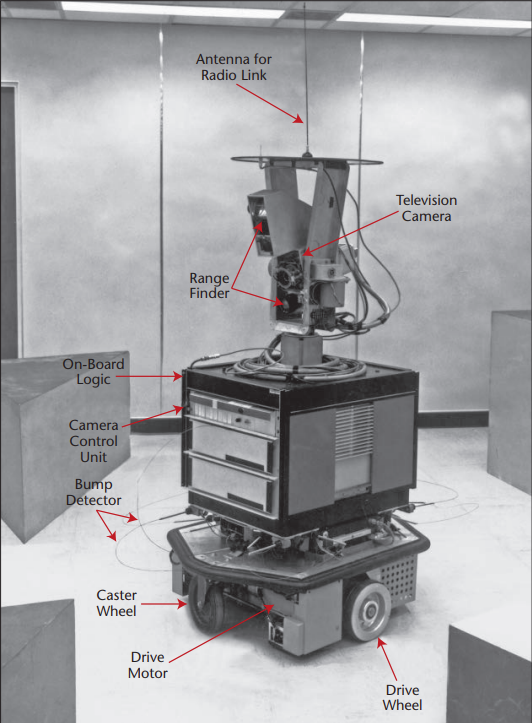
\includegraphics[width=0.25\textwidth]{Images/shakey.png}
    \caption{\textit{Shakey}.}
    \label{shakey}
    \vspace{-10pt}
\end{wrapfigure}
\end{comment}

Sus usos principales fueron la investigación en inteligencia artificial, robótica cognitiva 
y el desarrollo de planificación simbólica (\textit{STRIPS}) y experimentos de percepción, navegación y 
razonamiento. De hecho, la investigación realizada por el \textit{SRI} con \textit{Shakey}
obtuvo como resultado el algoritmo de búsqueda A* y los primeros algoritmos de
navegación y visión artificial. \\

La arquitectura de \textit{Shakey} seguía un modelo completamente centralizado y jerárquico, 
estructurado en capas de percepción, representación del mundo, planificación y ejecución, 
como se observa en la Figura 5 de \cite{Shakey}. Cada una de estas capas correspondía a un 
módulo específico del sistema de control y el flujo seguía la descomposición vertical clásica: 
sensación $\rightarrow$ percepción $\rightarrow$ modelo del mundo $\rightarrow$ planificación 
$\rightarrow$ acción. \\

La capa de ejecución estaba formada por las acciones de bajo nivel, que interactuaban 
directamente con el \textit{hardware}, y por las acciones intermedias basadas en tablas de 
Markov, responsables de comportamientos reactivos persistentes. La capa de planificación 
correspondía a \textit{STRIPS}, el planificador simbólico encargado de generar secuencias de 
acciones para alcanzar objetivos complejos. Finalmente, la capa de representación del mundo 
estaba asociada a \textit{PLANEX}, que supervisaba la ejecución del plan, detectaba errores, 
replanificaba cuando era necesario y mantenía la coherencia entre el estado simbólico y el 
estado real del entorno. \\

\begin{wrapfigure}{r}{0.32\textwidth}
    \centering
    \vspace{-10pt}
    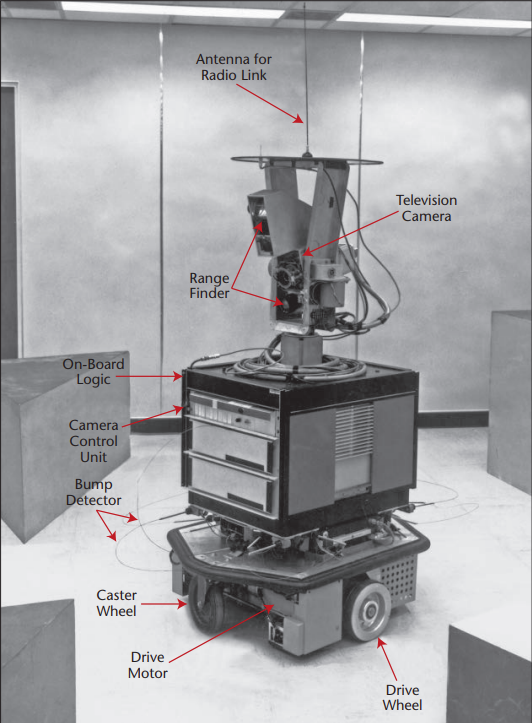
\includegraphics[width=0.28\textwidth]{Images/shakey.png}
    \caption{\textit{Shakey}.}
    \label{shakey}
    \vspace{-10pt}
\end{wrapfigure}

Shakey utilizaba un sistema de locomoción basado en dos ruedas motrices diferenciales (\textit{drive wheel}) 
y una rueda pasiva (\textit{caster wheel}) para mantener la estabilidad. El movimiento se controlaba variando
la velocidad relativa de las dos ruedas motrices, permitiendo avanzar, retroceder y girar 
sobre su propio eje.


\subsection*{Referencias}
\cite{Shakey} \fullcite{Shakey}.

\begin{comment}
\begin{figure}[H]
    \begin{center}
    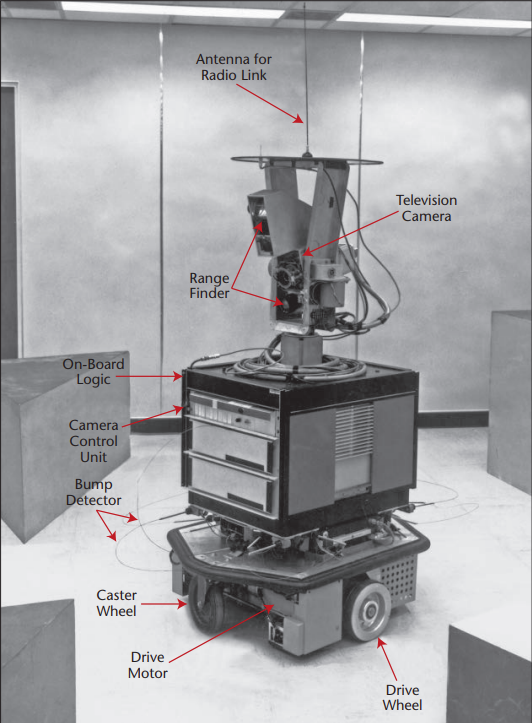
\includegraphics[scale=0.2, angle=0]{Images/shakey.png}
    \caption{\label{shakey}\textit{Shakey}.}
    \end{center}
\end{figure}
\end{comment}

\datos{color}{}{}
\subsection{\textit{TurtleBot 4}}
%\addcontentsline{toc}{section}{Ejercicio 1}

\textit{TurtleBot 4}, Figura \ref{turtlebot4}, es una plataforma móvil educativa y de investigación 
desarrollada en 2022 por 
\textit{Clearpath Robotics} y \textit{Open Robotics}. Está construida sobre la base del robot
móvil \textit{iRobot Create 3}, que actúa como plataforma de locomoción y sensorización de bajo nivel.
Sobre esta base se integra un conjunto de sensores modernos, como un \textit{LiDAR} 2D, una 
cámara \textit{RGB-D}, una \textit{IMU} y un ordenador principal, \textit{Raspberry Pi 4B},
que ejecuta los módulos de percepción, \textit{SLAM}, navegación y 
control dentro del ecosistema \textit{ROS2} (\textit{Robot Operating System}). 
Gracias a esta combinación, el \textit{TurtleBot 4}
es uno de los robots más utilizados en universidades y laboratorios para la 
enseñanza y experimentación en robótica móvil, así como para el desarrollo de aplicaciones 
prototipo. \\

Sus usos principales abarcan la educación en robótica y \textit{ROS2}, la investigación
en navegación autónoma y el diseño de algoritmos de \textit{SLAM}, percepción y planificación. \\

\begin{wrapfigure}{r}{0.4\textwidth}
    \centering
    \vspace{-10pt}
    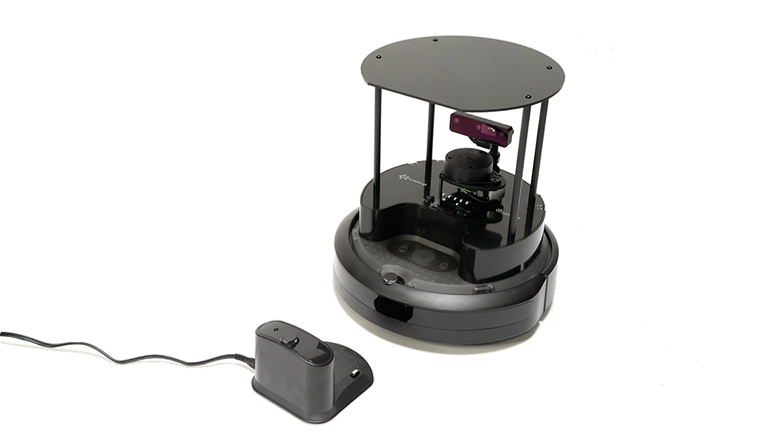
\includegraphics[width=0.4\textwidth]{Images/turtlebot.png}
    \caption{\textit{TurtleBot 4}.}
    \label{turtlebot4}
    \vspace{-10pt}
\end{wrapfigure}

Al igual que el robot \textit{Shakey}, el \textit{TurtleBot 4} presenta una arquitectura centralizada. 
Todos los sensores envían sus datos crudos a un único ordenador principal, encargado de ejecutar
los nodos de percepción, localización, construcción del mapa, planificación de rutas y control
del movimiento. La toma de decisiones se concentra en este módulo central, desde el que se 
envían directamente las órdenes a los actuadores. En consecuencia, no existe una distribución
de la inteligencia entre múltiples unidades de procesamiento, sino una estructura jerárquica
clásica basada en la secuencia percepción $\rightarrow$ planificación $\rightarrow$ acción. \\

Este robot también utiliza un sistema de locomoción diferencial compuesto por dos ruedas 
motrices laterales accionadas de manera independiente y una rueda libre trasera que 
proporciona estabilidad. Variando la velocidad relativa de las dos ruedas motrices, 
el robot puede avanzar, retroceder, girar sobre su eje y realizar maniobras precisas 
en entornos principalmente interiores.

\begin{comment}
\begin{figure}[H]
    \begin{center}
    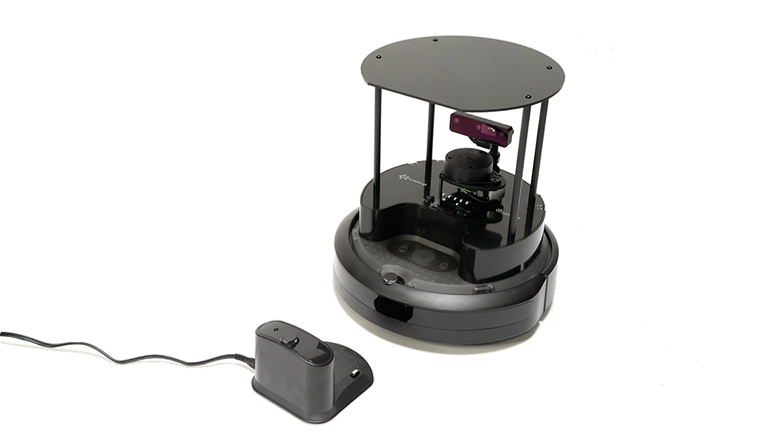
\includegraphics[scale=0.3]{Images/turtlebot.png}
    \caption{\textit{TurtleBot 4}.}
    \label{turtlebot4}
    \end{center}
\end{figure}
\end{comment}

\subsection*{Referencias}
\cite{TurtleBot4Clearpath} \fullcite{TurtleBot4Clearpath}.\\

\cite{TurtleBot4Manual} \fullcite{TurtleBot4Manual}.\\

\cite{iRobotCreate3} \fullcite{iRobotCreate3}.

\datos{color}{}{}
\subsection{\textit{RHex}}
\textit{RHex}, desarrollado inicialmente a comienzos de los años 2000 por un consorcio de
universidades liderado por la \textit{University of Michigan}, la \textit{University of Pennsylvania}
y \textit{McGill University}, Figura \ref{rhex}, es un robot hexápodo todoterreno diseñado para la
locomoción dinámica en terrenos irregulares. Su estructura ligera, su capacidad para desplazarse a
alta velocidad y su robustez mecánica lo convirtieron en una referencia en el estudio de la 
locomoción con patas y en el desarrollo de arquitecturas de control distribuidas y reactivas. 
\textit{RHex} emplea seis patas semirrígidas accionadas de manera independiente, lo que le permite 
correr, trepar, superar obstáculos y mantener la estabilidad incluso en superficies complejas. \\

Sus usos principales incluyen la investigación en locomoción bioinspirada, el estudio de
controladores reactivos, la exploración de terrenos no estructurados y el desarrollo de 
algoritmos de comportamiento distribuido. \textit{RHex} ha sido ampliamente utilizado en experimentos 
de campo, pruebas de movilidad extrema y estudios sobre estabilidad dinámica en robots de patas. \\

A diferencia de robots deliberativos clásicos como \textit{Shakey} o \textit{TurtleBot 4}, 
la arquitectura de \textit{RHex} es distribuida y se basa en la descomposición horizontal del 
problema. 
Cada pata dispone de controladores locales que procesan directamente la información sensorial 
y generan acciones motoras sin necesidad de un planificador central. Los módulos siguen
el principio de niveles de competencia: los controladores 
básicos garantizan la estabilidad y la locomoción elemental, mientras que capas superiores 
añaden comportamientos como evitar obstáculos, trepar o ajustar la postura. El comportamiento 
global del robot emerge de la interacción entre estos módulos, lo que permite respuestas rápidas y 
adaptativas ante cambios del entorno.\\

\begin{wrapfigure}{r}{0.34\textwidth}
    \centering
    \vspace{-10pt}
    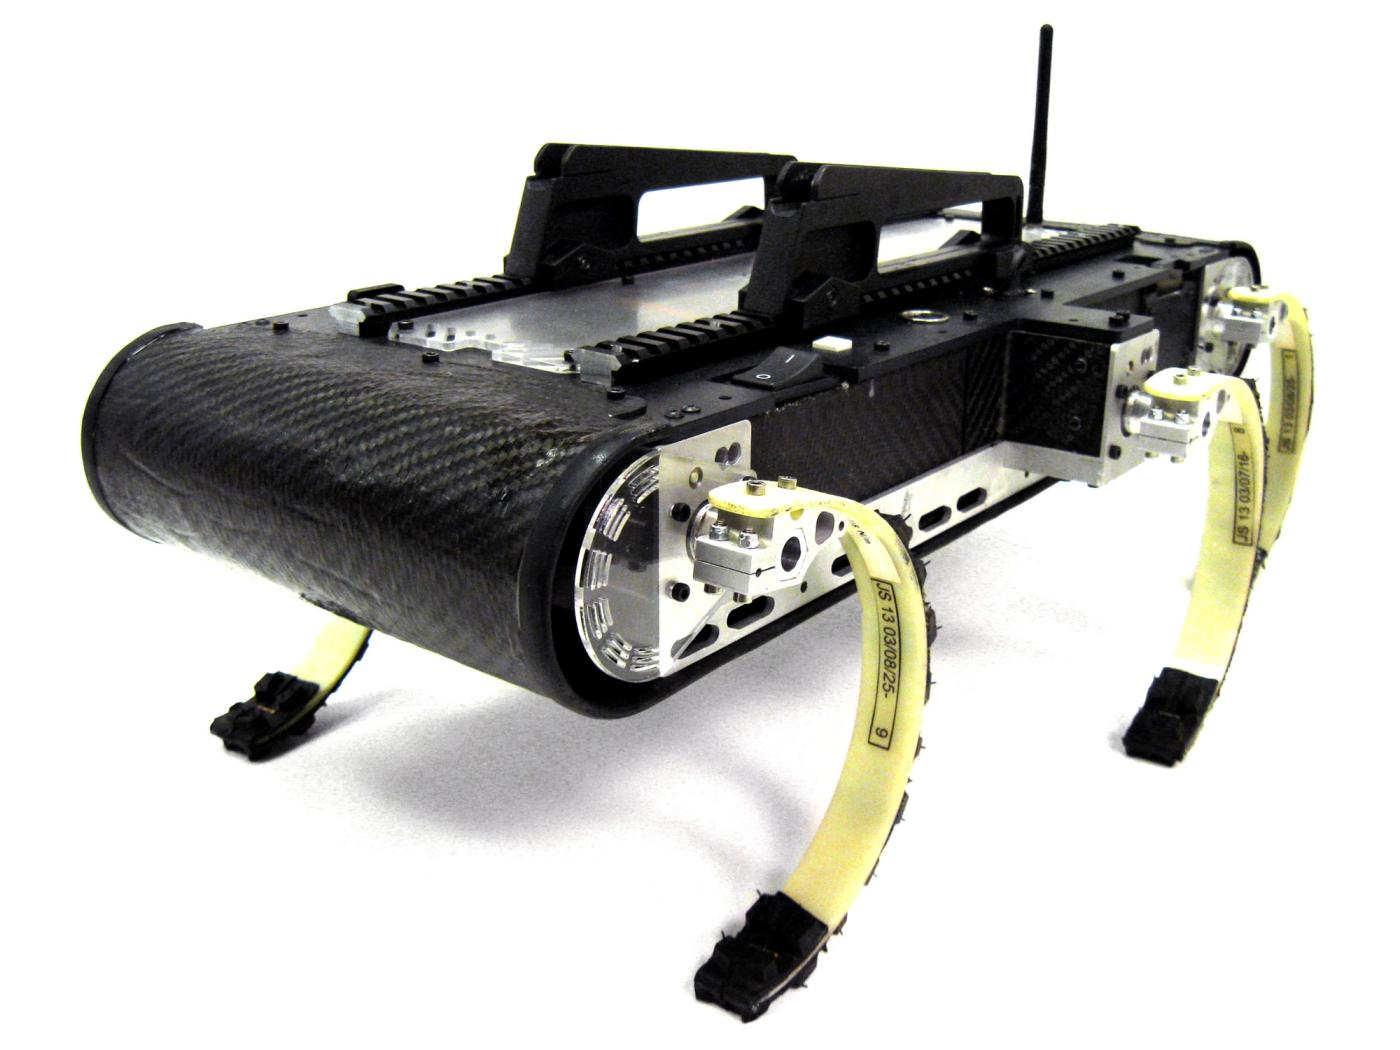
\includegraphics[width=0.34\textwidth]{Images/rhex.jpg}
    \caption{\label{rhex}\textit{RHex}.}
    \vspace{-10pt}
\end{wrapfigure}

\textit{RHex} utiliza un sistema de locomoción basado en seis patas rotatorias elásticas, 
cada una accionada por un motor independiente. La forma semicircular de las patas y su 
flexibilidad permiten generar tracción continua y absorber irregularidades del terreno. 
Variando la velocidad y fase relativa de las patas, el robot puede avanzar, girar, estabilizarse 
y ejecutar maniobras dinámicas como saltos o ascensos por superficies inclinadas. Este diseño 
mecánico, combinado con controladores distribuidos, le proporciona una movilidad excepcional 
en entornos donde los robots con ruedas o cadenas tienen dificultades. \\

\subsection*{Referencias}
\cite{doi:10.1177/02783640122067570} \fullcite{doi:10.1177/02783640122067570}.
\datos{color}{}{}
\subsection{\textit{MIT Cheetah}}
\textit{MIT Cheetah}, desarrollado por el \textit{Biomimetic Robotics Lab} del 
\textit{Massachusetts Institute of Technology} (\textit{MIT}), 
Figura \ref{cheetah}, es uno de los robots cuadrúpedos más influyentes en la investigación moderna 
sobre locomoción dinámica. Su primera versión funcional se presentó en 2012, y desde entonces ha 
evolucionado a \textit{Cheetah 2}, \textit{Cheetah 3} y \textit{Mini Cheetah}, convirtiéndose 
en una plataforma de referencia para el estudio del control híbrido, la planificación dinámica 
y la locomoción de alta velocidad. El robot integra actuadores eléctricos de alta potencia, 
sensores de torque, cámaras y sensores inerciales, junto con un ordenador central encargado de 
la percepción y la planificación. \\

Sus usos principales incluyen la investigación en control predictivo, locomoción dinámica, 
planificación de movimientos, aprendizaje por refuerzo y exploración autónoma. Gracias a su 
capacidad para correr, saltar, recuperar el equilibrio tras perturbaciones y desplazarse por 
terrenos irregulares, \textit{MIT Cheetah} ha sido ampliamente utilizado en experimentos de 
laboratorio y en estudios sobre estabilidad dinámica y control avanzado de cuadrúpedos. \\

A diferencia de los robots centralizados y distribuidos presentados anteriormente, 
\textit{MIT Cheetah} implementa una arquitectura de 
control híbrida. El ordenador central ejecuta los módulos de percepción, integración multisensorial,
planificación de trayectorias y control predictivo basado en modelos, siguiendo la descomposición 
vertical clásica. Sin embargo, cada articulación dispone de controladores locales que procesan 
directamente la información sensorial y generan respuestas rápidas para mantener la estabilidad, 
absorber impactos o corregir perturbaciones. Los niveles superiores planifican el movimiento global
mediante técnicas 
como el \textit{Model Predictive Control} (\textit{MPC}), mientras que los niveles inferiores garantizan la 
ejecución reactiva y segura del patrón de marcha. Esta combinación de planificación deliberativa 
y control reactivo, es decir, arquitectura híbrida, permite al robot adaptarse rápidamente a 
cambios del entorno. \\

\begin{wrapfigure}{r}{0.3\textwidth}
\centering
\vspace{-10pt}
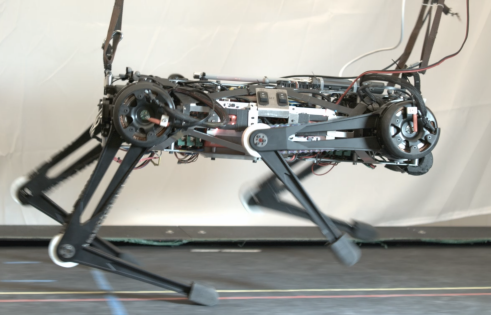
\includegraphics[width=0.3\textwidth]{Images/cheetah.png}
\caption{\label{cheetah}\textit{MIT Cheetah 3}.}
\vspace{-10pt}
\end{wrapfigure}

\textit{MIT Cheetah} utiliza un sistema de locomoción cuadrúpedo con doce grados de libertad, 
accionados mediante actuadores eléctricos de alta eficiencia y sensores de torque. La combinación 
de control de impedancia, estimación del estado corporal y planificación dinámica permite al robot
caminar, correr, saltar, girar con precisión y mantener la estabilidad ante perturbaciones externas. 
Su locomoción reactiva y su capacidad para ejecutar maniobras dinámicas complejas lo convierten en 
un ejemplo representativo de las arquitecturas híbridas modernas aplicadas a robots cuadrúpedos de 
alto rendimiento.

\subsection*{Referencias}
\cite{Cheetah2018} \fullcite{Cheetah2018}.\\
\cite{Cheetah2015} \fullcite{Cheetah2015}.
\datos{color}{}{}
\subsection{\textit{Crazyflie}}
\textit{Crazyflie}, desarrollado por \textit{Bitcraze AB} y presentado en 2013,
Figura~\ref{crazyflie}, es un nano–cuadricóptero modular y de código abierto
ampliamente utilizado en investigación y docencia. Su reducido tamaño, su arquitectura
flexible y su capacidad para integrar distintos módulos de control lo han convertido en una
plataforma de referencia para el estudio de control reactivo, navegación aérea y comportamientos emergentes en robots aéreos. El sistema integra una unidad inercial,
sensores de flujo óptico, barómetro y un microcontrolador encargado de ejecutar los módulos de
control de bajo nivel. \\

Sus usos principales incluyen la investigación en control distribuido a nivel de enjambre,
sistemas multi-robot, navegación reactiva, aprendizaje por refuerzo y experimentación en entornos interiores. Gracias a su
diseño abierto y a su modularidad interna, \textit{Crazyflie} se ha convertido en una herramienta
habitual en laboratorios de robótica aérea y en proyectos de investigación sobre comportamiento
colectivo. \\

\begin{wrapfigure}{r}{0.38\textwidth}
\centering
\vspace{-10pt}
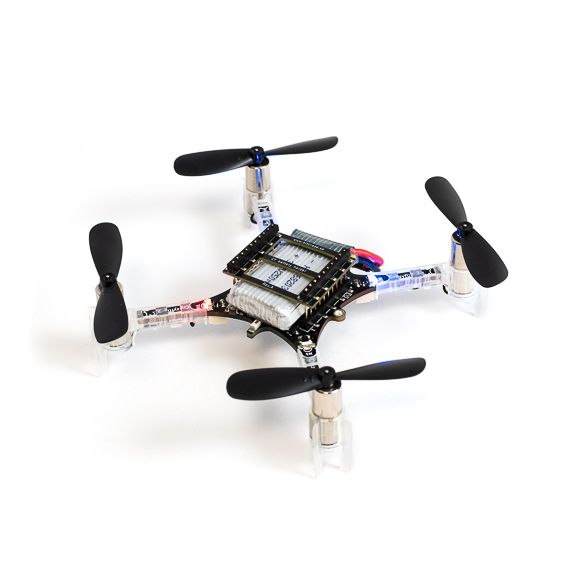
\includegraphics[width=0.34\textwidth]{Images/crazyflie.jpg}
\caption{\label{crazyflie}\textit{Crazyflie 2.1}.}
\vspace{-10pt}
\end{wrapfigure}

\textit{Crazyflie} implementa una arquitectura centralizada, en la que la
información fluye de forma vertical desde los sensores hacia los módulos 
de percepción y estimación, y desde estos hacia los módulos de control que 
generan las órdenes motoras. Un único microcontrolador ejecuta todos los 
niveles funcionales —estabilidad, control de acción, control de altura, 
evasión de obstáculos y estimación del estado—, de modo que ningún sensor 
ni actuador es gestionado de manera autónoma por módulos independientes. 
Estos no constituyen niveles de competencia.\\

\textit{Crazyflie} utiliza un sistema de locomoción aéreo basado en cuatro rotores controlados
de manera independiente. \\

\subsection*{Referencias}
\cite{BitcrazeWebsite} \fullcite{BitcrazeWebsite}. \\
\cite{7989376} \fullcite{7989376}.\\
\datos{color}{}{}

\subsection{Pez robot \textit{UJI–CIRTESU}}

El pez robot desarrollado por el \textit{Interactive and Robotic Systems Laboratory} (\textit{IRS-Lab}) 
de la \textit{Universitat Jaume I} (\textit{UJI}), en colaboración con el grupo \textit{CIRTESU},
Figura \ref{pezrobot}, 
representa una plataforma biomimética diseñada para la exploración y monitorización en 
entornos submarinos. El sistema fue presentado en las \textit{Jornadas de Automática 2025}, 
donde recibió el premio al mejor trabajo en Automática Marina. Su diseño se inspira en la 
locomoción ondulatoria de los peces, integrando electrónica embarcada, sensores y un 
mecanismo de propulsión basado en aletas flexibles. \\

Sus usos principales incluyen la investigación en robótica submarina, el estudio de 
locomoción biomimética, la monitorización ambiental en puertos y zonas costeras, y la 
experimentación con sistemas de comunicación acústica entre robots marinos. El pez robot 
ha sido empleado en pruebas reales en el puerto de Castellón, donde interactuó con un 
robot de superficie mediante un enlace acústico de baja tasa. \\

La arquitectura del sistema sigue un modelo completamente centralizado y jerárquico. 
El robot submarino ejecuta únicamente el control de bajo nivel asociado al movimiento 
de las aletas y la estabilización, mientras que la planificación, supervisión y toma de 
decisiones se realizan en un ordenador externo situado en el robot de superficie. 
La comunicación entre ambos se establece mediante un módem acústico, lo que refuerza 
la estructura maestro–esclavo del sistema. El flujo de control sigue la secuencia clásica: 
sensado local $\rightarrow$ transmisión acústica $\rightarrow$ planificación en superficie 
$\rightarrow$ envío de comandos $\rightarrow$ acción. \\

\begin{wrapfigure}{r}{0.4\textwidth}
    \centering
    \vspace{-10pt}
    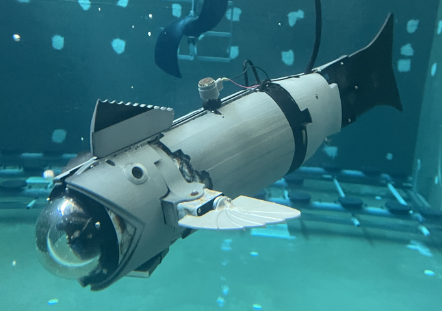
\includegraphics[width=0.36\textwidth]{Images/pez.png}
    \caption{Pez robot \textit{UJI–CIRTESU}.}
    \label{pezrobot}
    \vspace{-10pt}
\end{wrapfigure}

El método de locomoción se basa en una aleta de cola y dos laterales, todas accionadas por servomotores.
La aleta de cola genera un movimiento oscilatorio periódico. Este mecanismo produce una propulsión 
similar a la de los peces reales, permitiendo maniobrabilidad, eficiencia energética y 
movimientos suaves en el medio acuático. El diseño biomimético facilita la navegación en 
espacios reducidos y reduce el impacto ambiental respecto a los sistemas de hélice 
convencionales.

\subsection*{Referencias}

\cite{Puig2025FishRobot} \fullcite{Puig2025FishRobot}.\\
\cite{PortCastello2025PezRobot} \fullcite{PortCastello2025PezRobot}.

\datos{color}{}{}

\subsection{\textit{FLIR Kobra 725}}

El \textit{Kobra 725}, Figura \ref{kobra725}, desarrollado por \textit{Teledyne FLIR} a partir de 2021, es un robot terrestre 
de intervención equipado con un sistema de locomoción basado en orugas de alta tracción. 
Diseñado para operaciones de desactivación de explosivos (\textit{EOD}), reconocimiento, inspección 
y rescate, destaca por su capacidad para superar obstáculos, su modularidad y su elevada 
carga útil. Su arquitectura robusta y su movilidad lo convierten en una plataforma de referencia 
en robótica táctica moderna. \\

Sus usos principales incluyen la inspección remota en entornos peligrosos, la manipulación 
de objetos mediante su brazo robotizado, la exploración de zonas colapsadas, la vigilancia 
y la intervención en escenarios de riesgo químico, biológico o explosivo. Su despliegue es 
habitual en cuerpos de seguridad y equipos de emergencia. \\

La arquitectura \textit{software} del \textit{Kobra 725} sigue un modelo centralizado, con un ordenador embarcado 
que gestiona la percepción, el control de locomoción y la supervisión del sistema. El operador 
interactúa mediante una estación de control remota que envía comandos de alto nivel y recibe 
vídeo, telemetría y datos sensoriales. El robot integra cámaras \textit{HD}, sensores térmicos, \textit{IMU} y 
módulos de comunicación cifrada, permitiendo operación segura en tiempo real. \\

El método de locomoción se basa en un sistema de orugas de alta adherencia combinado con 
\textit{flippers} articulados que permiten subir escaleras, superar escombros y ajustar la 
postura del robot para mejorar la estabilidad. Este sistema proporciona movilidad fiable en 
terrenos irregulares, superficies resbaladizas y entornos no estructurados. \\

\begin{wrapfigure}{r}{0.32\textwidth}
    \centering
    \vspace{-10pt}
    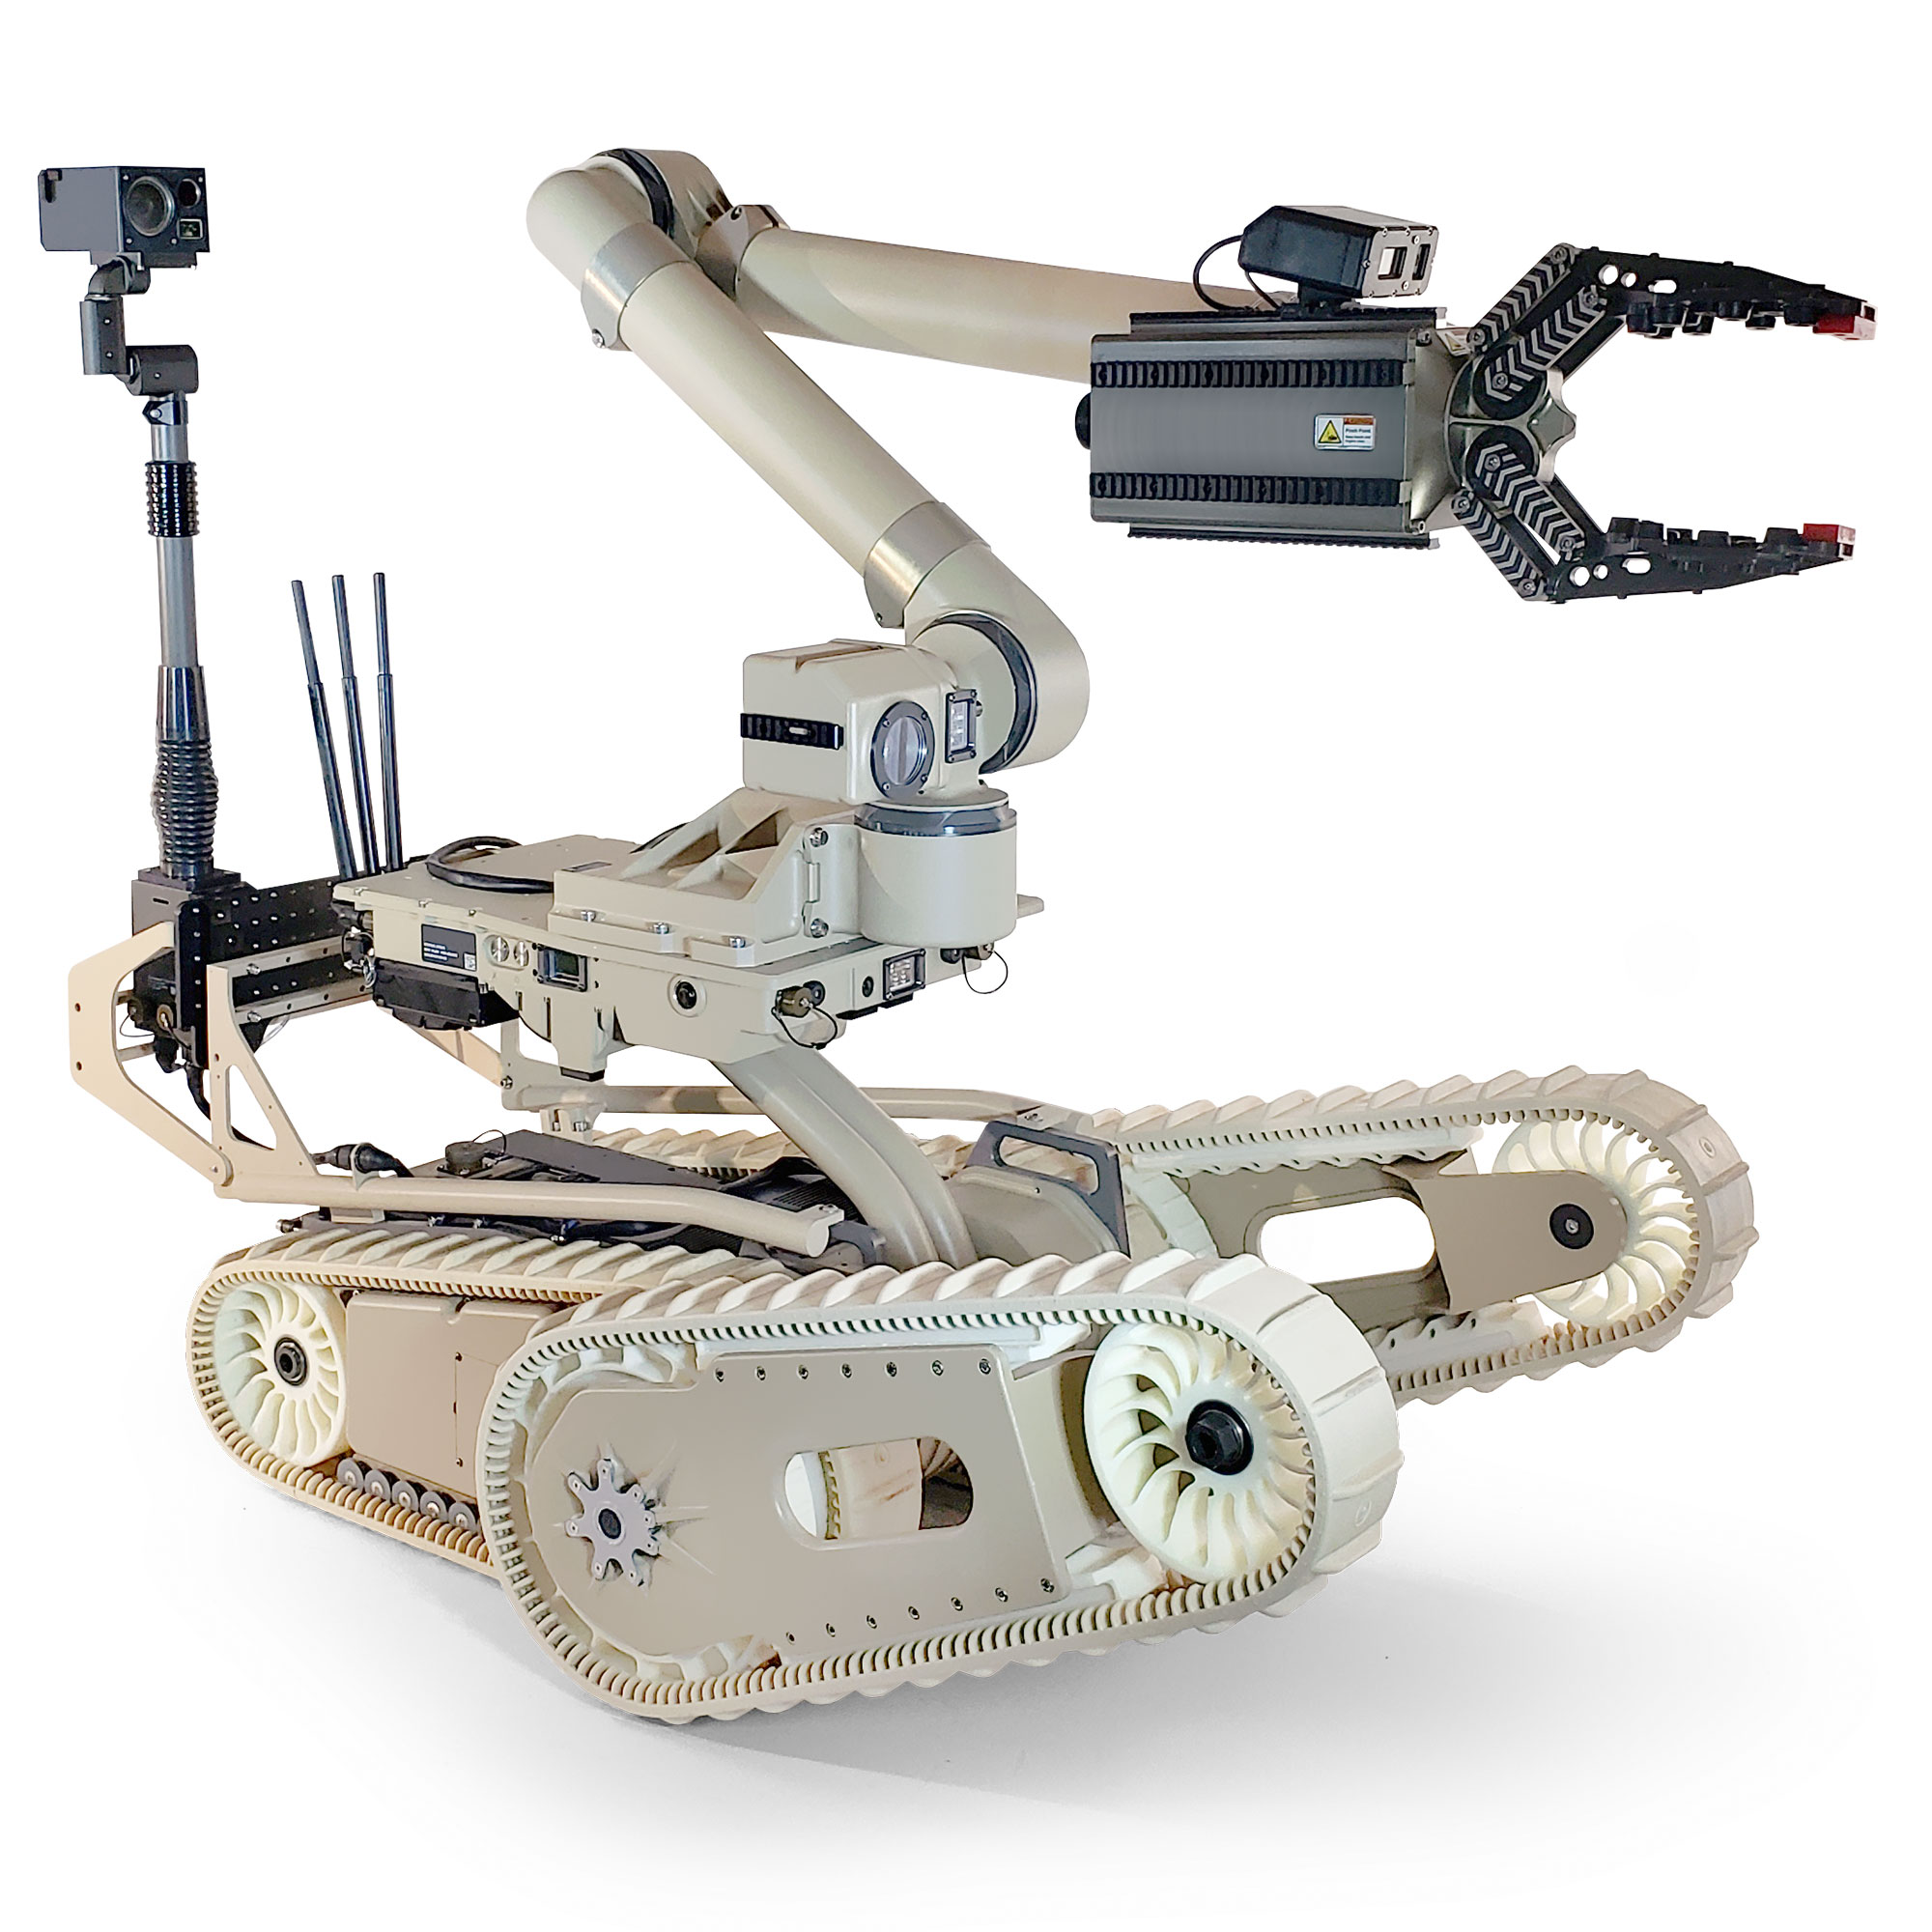
\includegraphics[width=0.28\textwidth]{Images/flirKobra725.jpg}
    \caption{\textit{FLIR Kobra 725}.}
    \label{kobra725}
    \vspace{-10pt}
\end{wrapfigure}

\subsection*{Referencias}

\cite{Kobra725Ref} \fullcite{Kobra725Ref}.

\datos{color}{}{}

\subsection{\textit{TIAGo}}

\textit{TIAGo} (acrónimo de \textit{Take It And Go}), Figura \ref{tiago}, es un robot colaborativo móvil desarrollado por 
\textit{PAL Robotics}, empresa con sede en Barcelona especializada 
en robótica de servicio y plataformas colaborativas, a partir de 2015 y ampliamente utilizado en investigación en robótica de 
servicio, interacción humano–robot y manipulación autónoma. Combina una base móvil diferencial u omnidireccional, 
uno o dos brazos manipuladores colaborativos de 7 grados de libertad cada uno y un torso elevable, lo que le permite 
realizar tareas complejas de navegación y manipulación en entornos humanos. \\

Sus usos principales incluyen la asistencia en entornos domésticos y hospitalarios, la 
manipulación colaborativa, la navegación autónoma en interiores, la investigación en 
interacción humano–robot, la percepción avanzada y la participación en competiciones 
robóticas como la \textit{RoboCup@Home}. Su versatilidad lo convierte en una plataforma 
estándar en numerosos laboratorios europeos. \\

\begin{wrapfigure}{r}{0.5\textwidth}
    \centering
    \vspace{-10pt}
    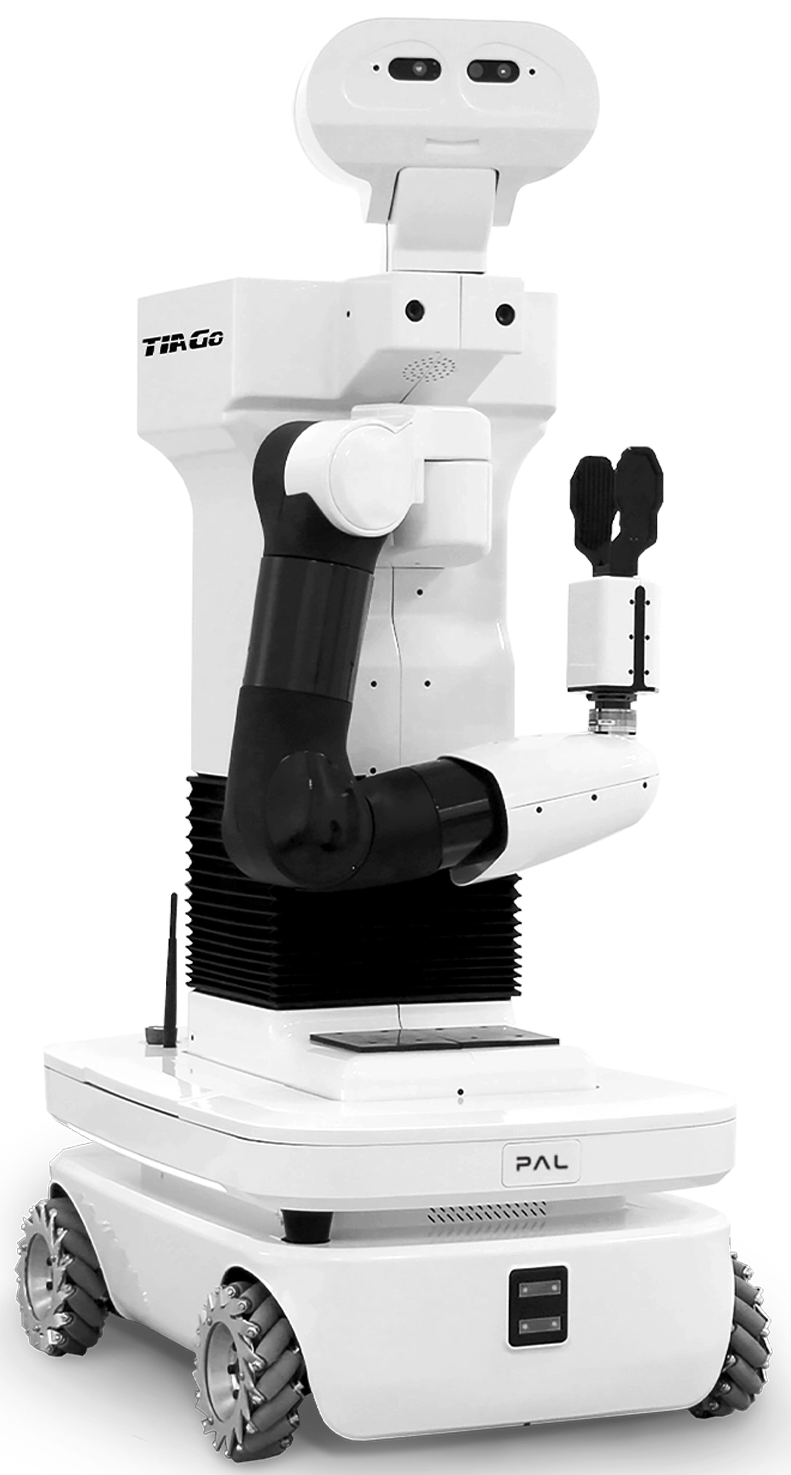
\includegraphics[width=0.2\textwidth]{Images/tiago.png}
    \caption{\textit{TIAGo}.}
    \label{tiago}
    \vspace{-10pt}
\end{wrapfigure}

La arquitectura del sistema es híbrida, combinando control centralizado para la planificación 
global y módulos distribuidos para la percepción, la navegación y el control del manipulador. 
El robot integra un ordenador embarcado de alto rendimiento que ejecuta \textit{ROS2} y gestiona 
la fusión sensorial, \textit{SLAM}, la planificación de trayectorias y la supervisión del sistema. 
Los controladores de bajo nivel del brazo, la base y el torso funcionan como nodos 
independientes, comunicándose mediante ROS2 y buses internos en tiempo real. \\

El método de locomoción se basa en una base móvil con ruedas diferenciales u omnidireccionales 
(según la configuración), equipada con sensores láser \textit{2D/3D}, cámaras \textit{RGB-D} y 
odometría. Esta base permite navegación autónoma, evitación de obstáculos y movimientos 
precisos en espacios estrechos. Los manipuladores colaborativos de 7 grados de libertad, 
accionados por motores eléctricos y 
reductores armónicos, permiten realizar tareas de manipulación segura junto a humanos.

\subsection*{Referencias}

\cite{Pags2016TIAGoTM} \fullcite{Pags2016TIAGoTM}.\\
\cite{TiagoRef} \fullcite{TiagoRef}.

\datos{color}{}{}

\subsection{\textit{Unitree G1}}

El \textit{Unitree G1}, Figura \ref{unitreeg1}, es un robot humanoide desarrollado por \textit{Unitree Robotics} a partir de 
2021 como plataforma de investigación en locomoción bípeda, manipulación y control dinámico. 
Su diseño compacto y ligero, junto con actuadores de alto par y sensores avanzados, lo 
convierten en un humanoide adecuado para tareas de navegación autónoma, interacción con 
objetos y experimentación en entornos reales. Su diseño modular permite integrar sensores adicionales, cámaras 
\textit{RGB-D}, \textit{LiDAR 3D} y herramientas de manipulación, adaptándose a múltiples escenarios de 
investigación y aplicaciones reales. \\\\

Sus usos principales incluyen la investigación en locomoción bípeda, control predictivo, 
aprendizaje por refuerzo, manipulación autónoma, interacción humano–robot y aplicaciones 
industriales ligeras. También se emplea como plataforma educativa y experimental en 
laboratorios de robótica humanoide debido a su coste relativamente bajo y su arquitectura 
abierta a nivel de software. \\

La arquitectura del \textit{G1} es híbrida: un ordenador central ejecuta la percepción,
la planificación de movimientos y la supervisión del sistema, mientras que cada 
articulación incorpora controladores locales responsables del control de par, posición y 
estabilidad. La comunicación entre módulos se realiza mediante buses de alta velocidad y 
\textit{ROS2}, integrando percepción, locomoción y manipulación en un sistema distribuido. \\

\begin{wrapfigure}{r}{0.4\textwidth}
    \centering
    \vspace{-10pt}
    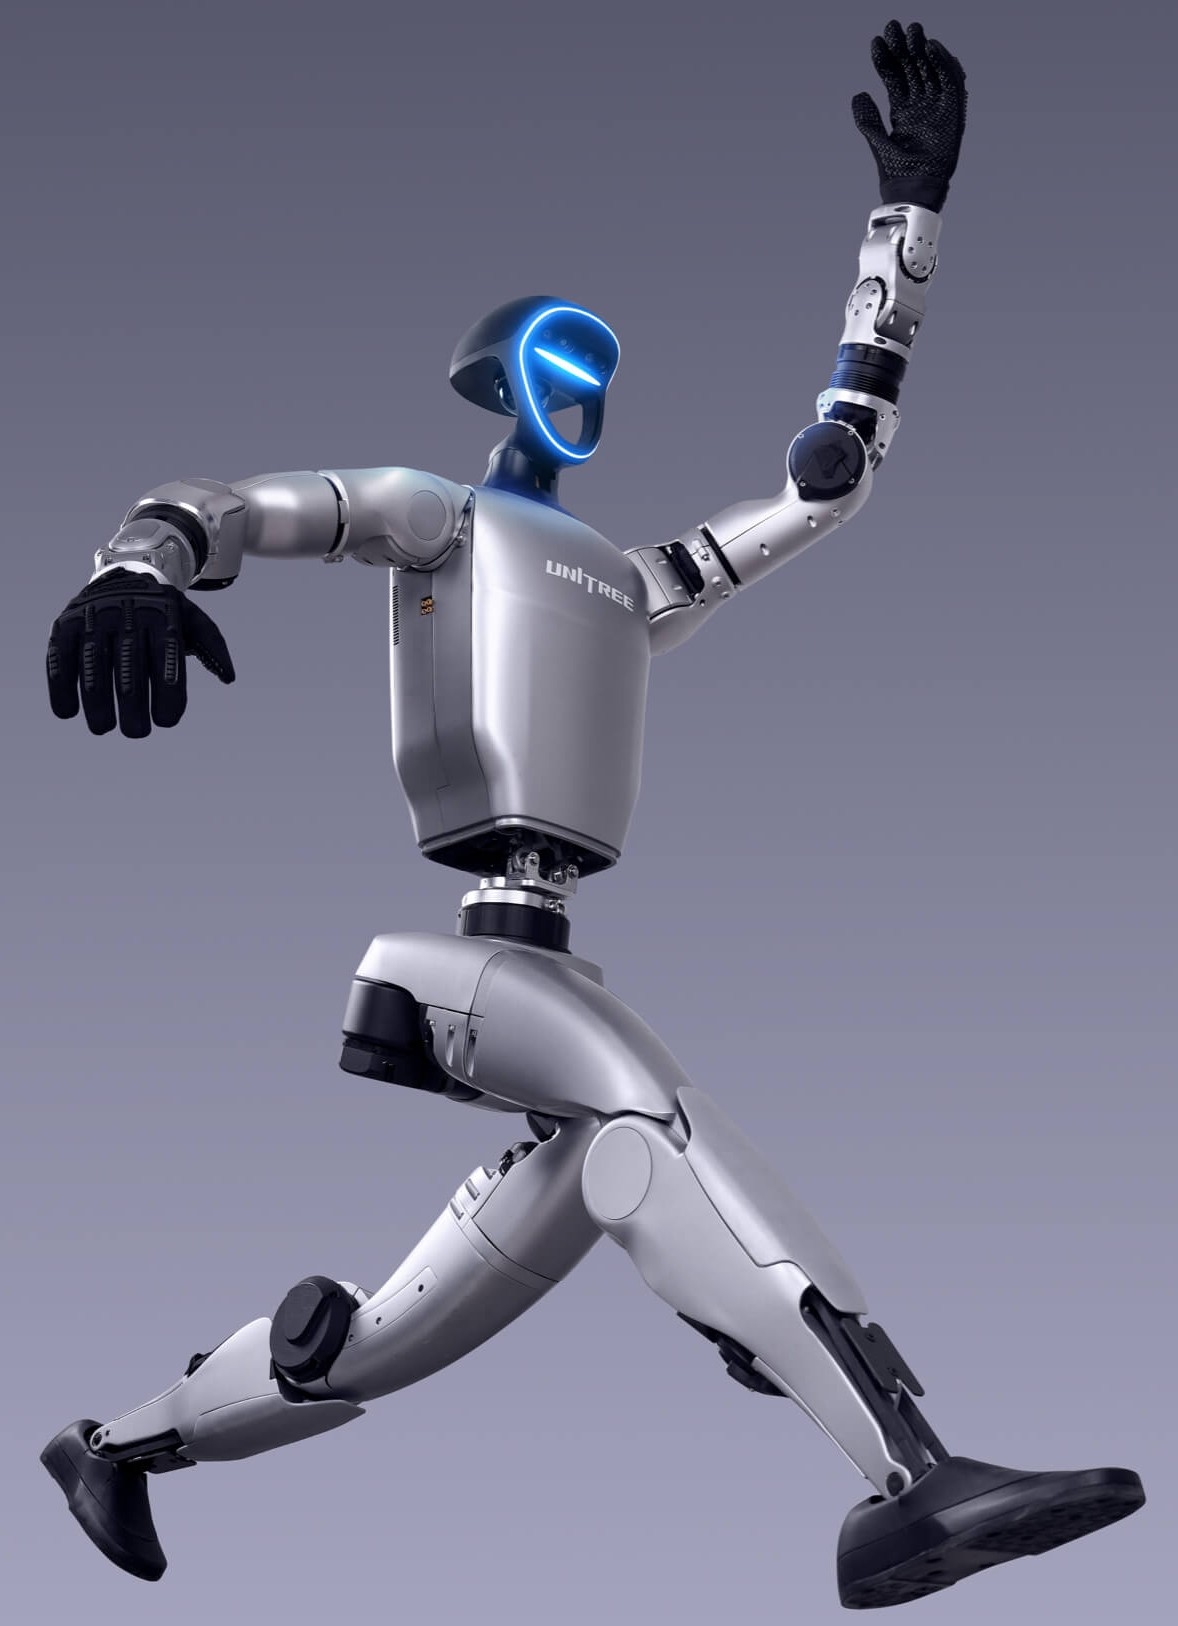
\includegraphics[width=0.2\textwidth]{Images/unitreeG1.jpg}
    \caption{\textit{Unitree G1}.}
    \label{unitreeg1}
    \vspace{-10pt}
\end{wrapfigure}

El método de locomoción se basa en dos piernas articuladas con múltiples grados de libertad, 
accionadas por motores eléctricos de alta potencia y controladas mediante algoritmos de 
control dinámico basados en modelos del centro de masa y control predictivo. Esta 
configuración permite caminar, mantener el equilibrio ante perturbaciones y ejecutar 
movimientos ágiles. El robot puede equiparse con manos robóticas para tareas de 
manipulación. \\

\subsection*{Referencias}

\cite{UnitreeG1Ref} \fullcite{UnitreeG1Ref}.


\newpage
\datos{color}{}{}
\printbibliography[title={Referencias}]
\addcontentsline{toc}{section}{Referencias}

\end{document}
